\documentclass{beamer}
\usetheme{Boadilla}
\usecolortheme{whale}
\setbeamertemplate{navigation symbols}{}

\usepackage{fontspec}
\usepackage{graphicx}
\graphicspath{{img/}}
\usepackage{listings}
\usepackage{xcolor}
\definecolor{light-gray}{gray}{0.92}
\usepackage{soul}
\sethlcolor{yellow}
\renewcommand<>{\hl}[1]{\only#2{\beameroriginal{\hl}}{#1}}
\makeatletter
\newcommand\SoulColor{%
  \let\set@color\beamerorig@set@color
  \let\reset@color\beamerorig@reset@color}
\makeatother
\SoulColor
\lstset{
    breaklines,
    basicstyle=\ttfamily\small,
    backgroundcolor=\color{light-gray},
    keywordstyle=\color{blue},
    stringstyle=\color{green!50!black},
    commentstyle=\color{gray}\ttfamily,
    moredelim=**[is][\color{red}]{@}{@},
    numbers=none,
    numberstyle=\tiny,
    numberblanklines=true,
    stepnumber=1,
    tabsize=4,
    numbersep=10pt,
    xleftmargin=0pt,
    showstringspaces=false,
}
\setlength{\fboxsep}{0pt}
\usepackage{polyglossia}
\setmainlanguage[babelshorthands,
                 spelling = new]{german}

\setcounter{tocdepth}{1} % Only sections in table of contents

\title[Statische Analyse]{Erstellung eines Frameworks zur statischen Analyse von Quelltexten}
\author{Jonas A. Wendorf}
\subject{Masterarbeit}
\institute{Hochschule Aalen}
\date{15.~April 2019}
\titlegraphic{
\includegraphics[scale=.3]{htw}}

\begin{document}
    \AtBeginSection{
        \begin{frame}
            \frametitle{Inhalt}
            \tableofcontents[currentsection]
        \end{frame}
    }

    \begin{frame}[plain]
        \titlepage%
    \end{frame}

    \begin{frame}
    	\frametitle{Inhalt}
        \tableofcontents%
    \end{frame}

    % Hier eigene Kapitel einfügen
    \section{Einleitung}
    \begin{frame}{\secname}
        \begin{itemize}
            \item Sicherheitsprüfungen können statisch oder dynamisch sein
            \item Dynamisch: Eingaben werden am laufenden Programm vorgenommen
            \item Statisch: Mögliche Eingaben werden anhand des Quelltextes nachvollzogen
            \item Entwicklung eines Frameworks zur statischen Analyse von Quelltexten
        \end{itemize}
    \end{frame}

    \subsection{Motivation}
        \begin{frame}{\secname: \subsecname}
            \begin{itemize}
                \item Dynamische Sicherheitsprüfungen sind kostenintensiv und zeitlich limitiert
                \item Statische Sicherheitsprüfungen können kostengünstig in die Entwicklungspipeline aufgenommen werden
                \item Existierende statische Codescanner sind
                    \begin{itemize}
                        \item teuer
                        \item schwer zu erweitern
                        \item teilweise inkompatibel mit neuen Versionen einer Programmiersprache
                        \item nicht für alle Programmiersprachen verfügbar
                    \end{itemize}
            \end{itemize}
        \end{frame}

    \section{Grundlagen}
    \subsection{Limitationen}
        \begin{frame}{\secname: \subsecname}
            \begin{itemize}
                \item »Alle interessanten Fragen über das Verhalten eines Programms sind unentscheidbar.« (M. Schwartzbach)
                \item Saloppe Zusammenfassung des Satzes von Rice
                \item Annäherung an das korrekte Ergebnis ist weiterhin möglich
            \end{itemize}
        \end{frame}

    \subsection{Ansätze}
        \begin{frame}{\secname: \subsecname}
            \framesubtitle{Einfache Stringsuche/reguläre Ausdrücke}
            \begin{itemize}
                \item Wird sehr schnell sehr kompliziert:\\
                      \lstinline@mysql_query\\((["'])SELECT .+ FROM .+ WHERE .+(?:\\=|\\s+I?LIKE\\s+|<>|>=?|<=?).+\\1\\)@
            \end{itemize}
            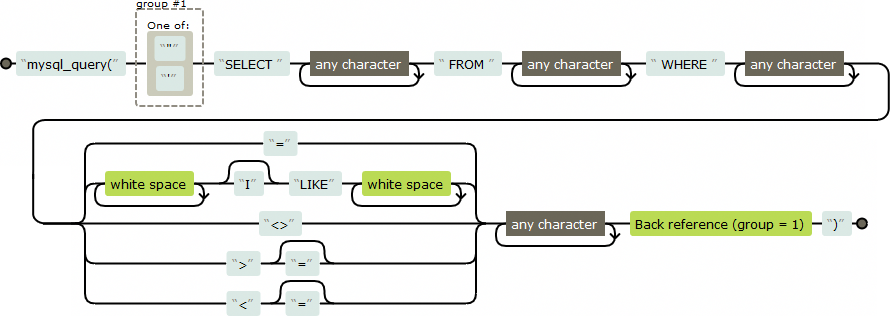
\includegraphics[keepaspectratio,height=\textheight,width=\columnwidth]{SQLi-RegEx.png}
        \end{frame}

        % \begin{frame}{\secname: \subsecname}
        %     \framesubtitle{Symbolische Ausführung}
        %     \begin{itemize}
        %         \item Programm wird simuliert
        %         \item Bedingungen werden mittels Constraint Solver getestet (SAT-Problem)
        %         \item Großes Problem: Pfadexplosion
        %         \item Erfordert exakte Definition des Programmablaufs
        %     \end{itemize}
        % \end{frame}

        \begin{frame}{\secname: \subsecname}
            \framesubtitle{Erstellung eines Parsers}
            \begin{itemize}
                \item Einfachere Abfragen als Stringsuche
                \item Keine Simulation des Laufzeitverhaltens
                \item[\textrightarrow] Kann unbekannte Bestandteile überspringen
                \item[\textrightarrow] Einfachere Erstellung eigener Sprachdefinitionen
                \item Für das Framework genutzter Ansatz
            \end{itemize}
        \end{frame}

    \subsection{Begriffe}
        \begin{frame}{\secname: \subsecname}
            \begin{itemize}
                \item Quelle (Source): Erzeugt benutzerdefinierte Eingaben
                \item Senke (Sink): Potentiell verwundbare Funktion
                \item Absicherung (Sanitizer): Sichert Eingaben für Senken ab
                \item Verschmutzung (Taint): Senke, die eine benutzerdefinierte Eingabe erhält
            \end{itemize}
        \end{frame}

    \section{Implementierung}
    \subsection{Vorgehensweise des Frameworks}
        \begin{frame}{\secname: \subsecname}
            \begin{enumerate}
                \item Quelltexte einlesen
                \item Passendes Modul auswählen
                \item Quelltexte parsen
                \item Regelsätze parsen
                \item Nach Schwachstellen suchen
                \item Codekomplexität analysieren
                \item Report erstellen
            \end{enumerate}
        \end{frame}

    % \subsection{Parsen der Quelltexte}
    %     \begin{frame}{\secname: \subsecname}
    %         \begin{itemize}
    %             \item PyParsing wird bevorzugt
    %             \item Grammatiken sind vergleichsweise einfach zu erstellen
    %             \item Eignet sich gut für einfachere Grammatiken
    %             \item[\textrightarrow] Für die Schwachstellensuche unwichtige Details werden ignoriert
    %             \item Andere Bibliotheken sind ebenfalls möglich, wenn die Ergebnisse an PyParsing angeglichen werden
    %         \end{itemize}
    %     \end{frame}

    % \subsection{Parsen der Regelsätze}
    %     \begin{frame}[fragile]{\secname: \subsecname}
    %         \begin{itemize}
    %             \item Regeln liegen im YAML-Format vor
    %             \item Werden mittels PyYAML geladen
    %             \item[\textrightarrow] Daten werden direkt in passenden Strukturen dargestellt
    %         \end{itemize}
    %         \begin{lstlisting}[gobble=16]
    %             {'OBJECT':
    %                 {'Methods':
    %                     [{'Methodname': 'METHODNAME',
    %                     'Parameters': [None, '$TAINT'],
    %                     'Comment': 'COMMENT'}]
    %                 }
    %             }
    %         \end{lstlisting}
    %     \end{frame}

    \subsection{Vorgehensweise bei der Suche nach Schwachstellen}
        \begin{frame}{\secname: \subsecname}
            \begin{enumerate}
                \item Parser ermittelt Methoden innerhalb der Datei
                \item Findet alle Variablen, die innerhalb der Methode verwendet werden
                \item Sucht nach möglichen Quellen, Senken oder Absicherungen
                \item Vergleicht die Eingabeparameter mit der Variablenliste
                \item[\textrightarrow] Schließt hardcodierte Methodenaufrufe aus
                \item Verfolgt Variablen zurück
                \item Informiert das Framework über neu hinzugekommene verwundbare Methoden
                \item Wiederholung bis keine neuen Ergebnisse geliefert werden
            \end{enumerate}
        \end{frame}

    \subsection{Variablenrückverfolgung}
        \begin{frame}[fragile]{\secname: \subsecname}
            \begin{itemize}
                \item Verfolgung der Variable »test« im Aufruf von \texttt{printf}
            \end{itemize}
            \begin{lstlisting}[gobble=16, escapechar=!]
                #include <stdio.h>
                !\hl<6>{int main(int argc, char * argv[]) \{}!
                    !\hl<5>{char * foo = argv[1];}!
                    !\hl<4>{char * bar = foo;}!
                    !\hl<3>{char * test = bar;}!
                    !\hl<2>{printf(test);}!
                }
            \end{lstlisting}
        \end{frame}

    \subsection{Exklusive Kontrollstrukturen}
        \begin{frame}[fragile]{\secname: \subsecname}
            \begin{itemize}
                \item Kontrollstrukturen, die wechselseitig exklusive Pfade erzeugen
                \item Beispiel: if/else
            \end{itemize}
            \begin{lstlisting}[gobble=16, escapechar=@]
                #include <stdio.h>
                int main(int argc, char* argv[]) {
                    @\colorbox{yellow}{if (0) \{}@
                        @\colorbox{yellow}{test();}@
                    } @\colorbox{green}{else if (2) \{}@
                        @\colorbox{green}{printf(argv[1]);}@
                    } @\colorbox{cyan}{else if (3) \{}@
                        @\colorbox{cyan}{printf("hallo\textbackslash{}n");}@
                    } @\colorbox{brown}{else \{}@
                        @\colorbox{brown}{printf("bye!\textbackslash{}n");}@
                    }
                    return 0;
                }
            \end{lstlisting}
        \end{frame}

%     \subsection{Komplexitätsprüfung}
%         \begin{frame}{\secname: \subsecname}
%             \begin{itemize}
%                 \item Nutzt zyklomatische Komplexität
%                 \item \( v(G) = e - n + 2 \)
%                 \item \( n \) sind die Knoten, \( e \) die Kanten
%                 \item Jede Anweisung ist ein Knoten und eine Kante
%                 \item Exklusive Kontrollstrukturen sind ein Knoten und zwei Kanten
%                 \item Schleifen sind ein Knoten und drei Kanten (Einstieg, Wiederholung, Ende)
%                 \item Gibt an, wie viele Testfälle maximal benötigt werden, um die Methode komplett zu testen
%                 \item Eher geringe Aussagekraft, aber gut als Indikator für mögliche Probleme geeignet
%             \end{itemize}
%         \end{frame}

    \section{Regelsätze}
    \subsection{Format}
        \begin{frame}[fragile]{\secname: \subsecname}
            \begin{itemize}
                \item Aufgebaut in YAML
                \item Unterschiedlich für Quellen und Senken
                \item[\textrightarrow] Senken haben optionalen Absicherungsblock
            \end{itemize}
            \begin{lstlisting}[gobble=16, escapechar=!]
                ---
                OBJEKTNAME:
                    Methods:
                    - Methodname: METHODENNAME
                      Parameters: [null, $TAINT, null]
                      Comment: KOMMENTAR
                      !\textcolor{gray!95}{Sanitizers:}!
                      !\textcolor{gray!95}{- OBJEKTNAME}!
                          !\textcolor{gray!95}{Methods:}!
                          !\textcolor{gray!95}{- Methodname: METHODNAME}!
                            !\textcolor{gray!95}{Parameters: []}!
                            !\textcolor{gray!95}{Comment: KOMMENTAR}!
            \end{lstlisting}
        \end{frame}

    \subsection{Beispielregel scanf}
        \begin{frame}[fragile]{\secname: \subsecname}
            \begin{itemize}
                \item \texttt{scanf} in C liest formatierten Text ein
                \item Erster Parameter ist Formatstring, darauffolgende Parameter sind Zielvariablen
            \end{itemize}
            \begin{lstlisting}[gobble=16]
                ---
                null:
                    Methods:
                    - Methodname: scanf
                      Parameters: [null, $TAINT]
                      Comment: Reads formatted input from stdin
            \end{lstlisting}
        \end{frame}

    \subsection{Beispielregel printf}
        \begin{frame}[fragile]{\secname: \subsecname}
            \begin{itemize}
                \item \texttt{printf} in C gibt formatierten Text aus
                \item Bei nur einem Parameter wird dieser als Formatstring erkannt
                \item Benutzer kann eigene Formatstrings einfügen, um Daten zu offenbaren und Speicher zu ändern
            \end{itemize}
            \begin{lstlisting}[gobble=16]
                ---
                null:
                    Methods:
                    - Methodname: printf
                      Parameters: [$TAINT]
                      Comment: Format string vulnerability.
            \end{lstlisting}
        \end{frame}

    \section{Beispielreport}
    % \subsection{Mögliche Formate}
    %     \begin{frame}{\secname: \subsecname}
    %         \begin{itemize}
    %             \item Ausgabe ist möglich als reiner Text (auf der Konsole oder in einer Datei gespeichert),
    %             \item im Markdown-Format oder
    %             \item als HTML-Datei mit eigenem CSS und JavaScript
    %         \end{itemize}
    %     \end{frame}

    \subsection{Verwendete Software}
        \begin{frame}{\secname: \subsecname}
            \begin{itemize}
                \item Terminaldateimanager cfiles (Stand vom 17. Januar 2019)
                \item In C geschrieben
                \item Typische Sicherheitslücken
                \item Schwachstellen mittlerweile korrigiert
                \item Insgesamt mit vier Senken-Regeln 24 Verschmutzungen und 31 Senken gefunden
                \item Demo-Video
            \end{itemize}
        \end{frame}

    \subsection{Erkannte Verschmutzungen}
        \begin{frame}[fragile]{\secname: \subsecname}
            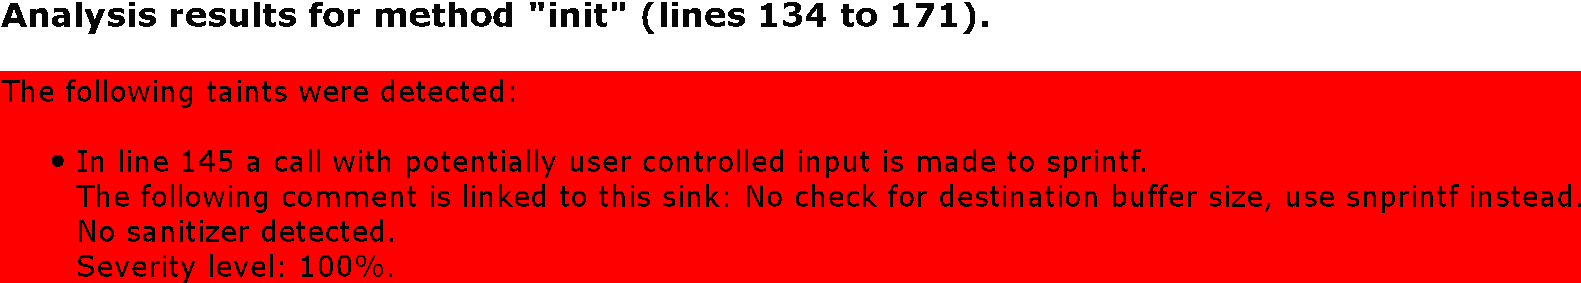
\includegraphics[keepaspectratio,height=\textheight,width=\columnwidth]{init-taint.pdf}
            \begin{lstlisting}[gobble=16, escapechar=!]
                char editor[20];
                void init()
                {
                    ...
                    // Set the editor
                    if( getenv("EDITOR") == NULL)
                        sprintf(editor, "%s", "vim");
                    else
                        !\colorbox{yellow}{sprintf(editor, "\%s", getenv("EDITOR"));}!
                    ...
                }
            \end{lstlisting}
        \end{frame}

    \subsection{Erkannte Senken}
        \begin{frame}[fragile]{\secname: \subsecname}
            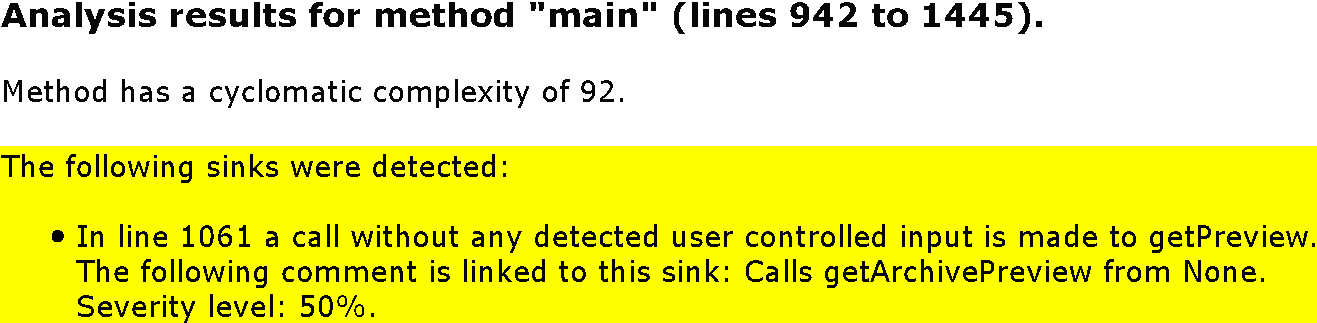
\includegraphics[keepaspectratio,height=\textheight,width=\columnwidth]{main-sink.pdf}
            \begin{lstlisting}[gobble=16, escapechar=!]
                int main(int argc, char* argv[]) {
                    ... !\colorbox{yellow}{getPreview(next\_dir,maxy,maxx/2+2);}! ...
                }
                void getPreview(char *filepath, int maxy, int maxx) {
                    ... !\colorbox{yellow}{getArchivePreview(filepath, maxy, maxx);}! ...
                }
                getArchivePreview(char *filepath, int maxy, int maxx) {
                    ... !\colorbox{yellow}{sprintf(temp\_dir,"atool -lq \textbackslash{}"\%s\textbackslash{}"\ > \textasciitilde/.cache/}!
                    !\colorbox{yellow}{cfiles/preview",filepath);}! ...
                }
            \end{lstlisting}
        \end{frame}

    \section{Fazit}
    \begin{frame}{\secname}
        \begin{itemize}
            \item Statische Analyse ist kein Allheilmittel
            \item Trotzdem können viele Schwachstellen bereits mit wenigen Regeln gefunden werden
            \item Eigene Regeln und sogar Module erstellen ist (vergleichsweise) einfach
            \item[\textrightarrow] Auch exotische Sprachen können getestet werden, kein Update des Herstellers notwendig
            \item Kann einfach in den Entwicklungsprozess eingebunden werden
        \end{itemize}
    \end{frame}

\end{document}
